\chapter{Environnement professionnel}

\section{L'entreprise}

\textbf{WeVii} est une Entreprise de Service du Numérique (ESN) créée en 2010 sous le nom d’AFIB Décision.
Son activité tournait autour de l’informatique décisionnelle.
En 2014, l’entreprise amorce un premier virage et se renomme \textbf{AFIB Services},
élargissant son activité à tous les services digitaux, et pas seulement au décisionnel. En 2019, face à des difficultés financières, l’entreprise est reprise par \textbf{Pascal Perigault} et \textbf{Romain Lavielle}, et devient \textbf{WeVii}.

\subsection{Évolution}

D’une situation critique avec quatre collaborateurs, l’entreprise s’est transformée pour atteindre aujourd’hui soixante-quinze collaborateurs répartis sur deux sites, Bordeaux et Lille, réalisant un chiffre d’affaires de sept millions d’euros.

\bigskip

\textbf{WeVii} est actuellement un groupe composé de huit entreprises :
\begin{itemize}
    \item Trois holdings : \textbf{Carat Conseil}, \textbf{Faerie Consulting}, et \textbf{WeVii Holding}.
    \item Les sociétés filles : \textbf{WeVii Bordeaux}, \textbf{WeVii Innovation}, \textbf{WeVii Paris}, \textbf{WeVii Lille}, et \textbf{WeVii Tech}.
\end{itemize}

\section{Les grandes dates}
\begin{figure}[H]
    \centering
    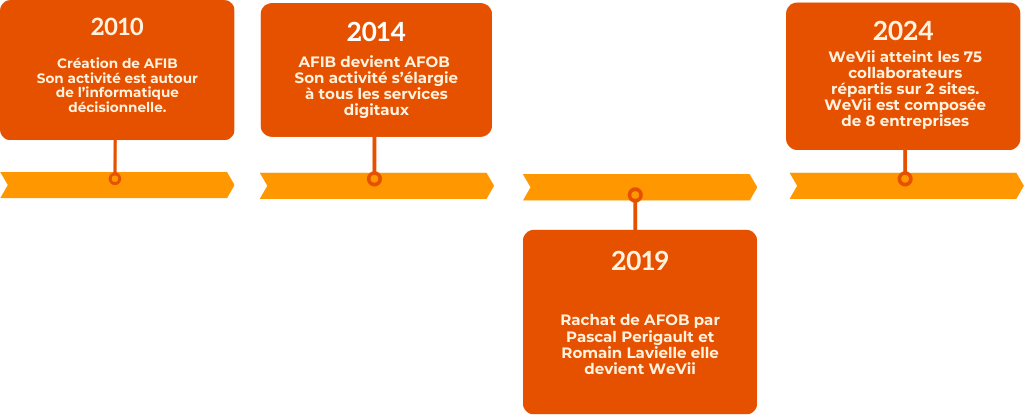
\includegraphics[width=\textwidth]{image/lesGrandesDates}
    \caption[Les grandes dates]{Les grandes dates de l'entreprise}
    \label{fig:grandes_dates}
\end{figure}

\section{Ma place dans l'entreprise}

Dans le cadre de cette transformation, \textbf{WeVii} lance des projets, dont un projet nommé \textbf{« TDC » (Tree Digital Cloud)}, porté par une nouvelle entreprise, \textbf{WeVii Innovation}, une JEI (Jeune Entreprise Innovante).
C’est pour ce projet, en tant que salarié de \textbf{WeVii Bordeaux}, que j’interviens dans le cadre de mon apprentissage.

\section{Organigramme de l'entreprise}
\begin{figure}[H]
    \centering
    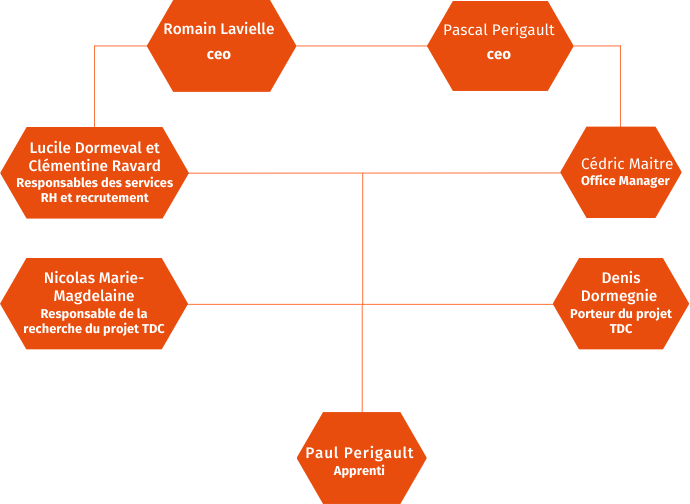
\includegraphics[width=\textwidth]{image/organigrammeEntreprise}
    \caption[Organigramme de l'entreprise]{Organigramme de l'entreprise}
    \label{fig:organigramme_entreprise}
\end{figure}

\section{Organisation de l'entreprise}

L'organisation du groupe est la suivante :
\begin{itemize}
    \item \textbf{Pascal Perigault} et \textbf{Romain Lavielle} sont les CEO.
    \item \textbf{Grégory Lacombe}, associé, dirige \textbf{WeVii Tech}, filiale de WeVii, nouvellement créée et spécialisée dans les métiers du cloud, de la sécurité et des opérations.
    \item \textbf{Lucile Dormeval} et \textbf{Clémentine Ravard} sont responsables des services RH et recrutement.
    \item \textbf{Cédric Maitre} est l'Office Manager (il dirige tout le back office).
    \item Les fonctions financières et paies sont sous-traitées par un cabinet spécialisé.
    \item \textbf{Nicolas Marie-Magdelaine}, Docteur en informatique, est responsable de la recherche du projet TDC. Il pilote mon activité technique.
    \item \textbf{Denis Dormegnie} est le porteur du projet TDC. Il pilote également mes projets.
\end{itemize}

\section{La vie en entreprise}

Durant la formation, mon outil de travail était un ordinateur portable MacBook Air fourni par l’entreprise.
J’ai été en grande partie en télétravail, bien que parfois je descendais à Bordeaux pour voir mes collègues et participer à la vie quotidienne et professionnelle de l’entreprise, afin de mieux m'intégrer.

\bigskip

Pour communiquer, nous utilisons \textbf{Teams}, un logiciel conçu par Microsoft permettant d’envoyer des messages, de faire des réunions à distance et de faciliter la communication inter-entreprise.
Malgré la distance, j’ai eu la chance de participer à la vie de l’entreprise, notamment en étant présent en visioconférence aux \textbf{WeTalkTech}, un podcast en direct où chaque intervenant présente une technologie ou un projet.

\bigskip

Les tâches m’étaient fournies par le chercheur, mais j’avais la possibilité d’ajouter une part de créativité.
J’utilisais la méthodologie \textbf{DevOps} pour construire et déployer mes projets tout en ayant une approche minimaliste apportée par le chercheur. Elles étaient sous forme de fonctionnalités et sous contraintes de temps, ce qui signifie que pour chaque élément à ajouter à l’application, nous estimons un temps pour le réaliser.

\clearpage
